% Source : http://tex.stackexchange.com/q/81812/86

\documentclass{standalone}
\usepackage{tikz}
\usetikzlibrary{hobby,decorations.markings}
\usepackage{graphicx}

\begin{document}
\begin{tikzpicture}
\draw[
  postaction={
    decorate,
    decoration={
      markings,
      mark=between positions 0 and 1 step 0.2 with
      {
        \node[transform shape] {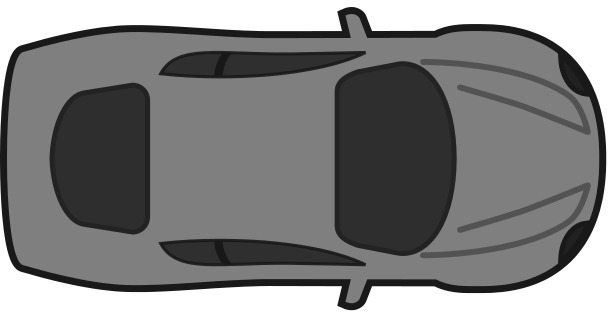
\includegraphics[width=.5cm]{car}};
      }
    }
  }
]
(0,0) to[out angle=0,in angle=180,curve through={(1,.9) .. (2,0) .. (3,.5)}] (4,0);
\end{tikzpicture}
\end{document}